 %\chapter{Background}
\section{Background \& Theoretical Basics }

In this chapter, we provide high-level explanations of the most important aspects and comprehensive understanding of the foundational theories and principles that make query optimization and materialized views effective. The concrete basics needed are explained the respective section along the thesis.

%some basics of the Database particularly distributed database.Then an overview of materialized view as query processing technique. later,we will discuss various methods and algorithms to about materialized view and Finally we discuss related work.
\subsection{ Database System}

\begin{definition}
A database is an organized collection of data or a type of data store based on the use of a database management system(DBMS), the software that enables the creation, modification and the database itself to capture and analyze the data.\end{definition}\vspace{.4cm}
A database in SQL Server is made up of a collection of tables that stores a specific set of structured data. A table contains a collection of rows, also refereed to as records or tuples and columns also referred to as attributes. Each column in the table is designed to store a certain type of information, for example: dates, names, dollar and numbers.\cite{williamdassafmsft-2024} Scalability, security, high availability, Network latency, fault tolerance these are the key characteristics of databases. There are two distinct types of databases: Homogeneous and heterogeneous databases.

\begin{itemize}
    \item \textbf{Homogeneous database:} In a homogeneous distributed database, the machines, nodes, servers, or sites store the same data, use the same data model, work with the same operating system, and share the same distributed database management system (DDBMS) or occasionally multiple types of DDBMS from the same vendor.\cite{mongodb-no-date}
    \item \textbf{Heterogeneous databases:} In a heterogeneous distributed database, different sites can use different schema and software that can lead to problems in query processing and transactions. Also, a particular site might be completely unaware of the other sites. Different computers may use a different operating system and different database applications. They may even use different data models for the database. Hence, translations are required for different sites to communicate.\cite{geeksforgeeks-2023}
\end{itemize}

\subsection{Query Processing }
A query is a request sent to a database for data retrieval. Specific conditions are passed in a query to match and retrieve relevant data. SQL (Structured Query Language) is used to write these queries to extract information from relational databases. The query process involves translating high-level queries into low-level expressions suitable for the file system, optimizing the query, and executing it to obtain the result. The steps involved in the execution of a query are as follows:\cite{wwwnaukricom-no-date}\\
\begin{figure}[h]
    \centering
    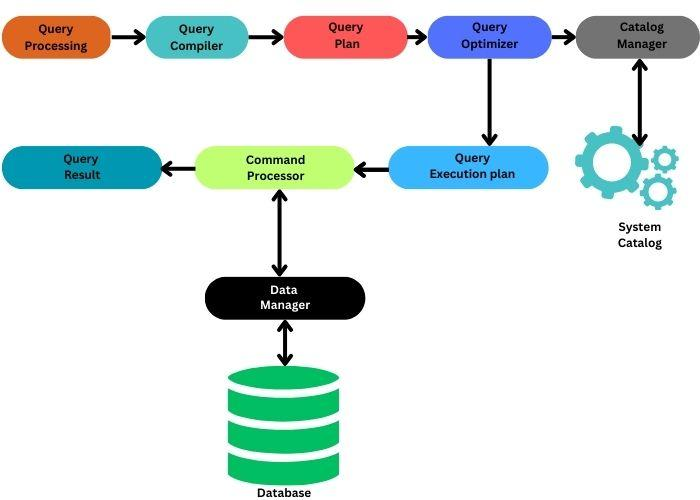
\includegraphics[width=0.5\textwidth]{Figure/Flow of QueryProcessing.jpg}
    \caption{The flow of query processing in DBMS.}
    \label{fig:my_image}
\end{figure}
\begin{enumerate}
\item \textbf{Parser:} Query parsing is the first step in query processing. In this steps, database performs the following checks- Syntax,semantic and shared pool check,after converting the query into relational algebra.\cite{wwwnaukricom-no-date}
    \begin{enumerate}
        \item \textbf{Syntax check:} A query is checked for syntax error.It concludes syntactic validity. Example:\\
        % Define colors
\definecolor{codegreen}{rgb}{0,0.6,0}  % Green for comments
\definecolor{codegray}{rgb}{0.5,0.5,0.5}  % Gray for numbers
\definecolor{codepurple}{rgb}{0.58,0,0.82}  % Purple for strings
\definecolor{backcolour}{rgb}{0.95,0.95,0.92}  % Light gray background
\definecolor{bordercolor}{rgb}{0.7,0.7,0.7}  % Left border color (gray)
\definecolor{codeblue}{rgb}{0,0,0.8}  % Blue for SQL keywords

\lstdefinelanguage{MySQL}{
    keywords={SELECT, FROM, WHERE, JOIN, ON, INNER, OUTER, LEFT, RIGHT, FULL, GROUP, BY, ORDER, ASC, DESC, AS, COUNT, SUM, AVG, MAX, MIN, DISTINCT, INSERT, INTO, VALUES, UPDATE, SET, DELETE, CREATE, TABLE, PRIMARY, FOREIGN, KEY, DEFAULT, NULL, NOT, CHECK, CONSTRAINT, INDEX, VIEW, MATERIALIZED, PROCEDURE, FUNCTION, TRIGGER, DATABASE, ALTER, DROP, EXEC, IF, EXISTS, UNION, ALL, CASE, WHEN, THEN, ELSE, END, CAST, CONVERT, LIKE, IN, BETWEEN, AND, OR, HAVING, LIMIT, OFFSET},
    sensitive=false,
    morestring=[b]',  % String in single quotes
    morestring=[b]"   % String in double quotes
}
\captionsetup[lstlisting]{font=small}
\lstdefinestyle{sqlstyle}{
    backgroundcolor=\color{backcolour},   
    commentstyle=\color{codegreen},  % Comments in green
    keywordstyle=\bfseries\color{codeblue},  % ✅ SQL Keywords in Blue & Bold
    numberstyle=\scriptsize\color{codegray},  % Row numbers in gray
    stringstyle=\color{codepurple},  % Strings in purple
    basicstyle=\ttfamily\footnotesize,
    breaklines=true,
    captionpos=b,
    numbers=left,      % ✅ Enables row numbers on the left
    stepnumber=1,      % ✅ Row numbers increment by 1
    firstnumber=1,     % ✅ Starts numbering at 1
    numbersep=8pt,     % ✅ Increases space between numbers and SQL code
    xleftmargin=3em,   % ✅ Ensures space inside the left border
    frame=single,      % ✅ Keeps a single border (left-aligned)
    framesep=5pt,      % ✅ Ensures space inside the frame
    rulesepcolor=\color{bordercolor},  % ✅ Matches row numbers with left border
    rulecolor=\color{bordercolor},  % ✅ Sets left border color
    language=MySQL  % ✅ Uses SQL keyword highlighting
}



\begin{lstlisting}[style=sqlstyle, caption={SQL query to check syntax}]
SQL>SELECT * form employees;SELECT * form employees * error at line 1:
FROM   keyword NOT found
WHERE  expected
\end{lstlisting}
          Here error of wrong spelling of FROM is given by this check.
        \item \textbf{Semantic check:} It checks whether the statement is meaningful or not. Example: Query contains a table name which doesn't exist\\
        
\definecolor{dkgreen}{rgb}{0,0.6,0}
\definecolor{gray}{rgb}{0.5,0.5,0.5}
\definecolor{mauve}{rgb}{0.58,0,0.82}
\lstset{language=SQL,
  basicstyle={\small\ttfamily},
  belowskip=3mm,
  breakatwhitespace=true,
  breaklines=true,
  classoffset=0,
  columns=flexible,
  commentstyle=\color{dkgreen},
  framexleftmargin=0.25em,
  frameshape={}{yy}{}{}, %To remove to vertical lines on left, set `frameshape={}{}{}{}`
  keywordstyle=\color{blue},
  numbers=none, %If you want line numbers, set `numbers=left`
  numberstyle=\tiny\color{gray},
  showstringspaces=false,
  stringstyle=\color{mauve},
  tabsize=3,
  xleftmargin =1em
}
         \begin{lstlisting}
         SQL> SELECT * FROM nonexistent_table;
         SELECT * FROM nonexistent_table
              *
        ERROR at line 1:
        ORA-00942: table or view does not exist
        FROM keyword not found where expected
        \end{lstlisting}
        A syntactically correct statement can fail a semantic check, as shown in the following example of a query of a nonexistent table.\cite{Oracle}
        \item \textbf{Shared pool check:} During the parse, the database performs a shared pool check to determine whether it can skip (hash code )resource-intensive steps of statement processing. Every query posses a hash code..
        % Define colors
\definecolor{codegreen}{rgb}{0,0.6,0}  % Green for comments
\definecolor{codegray}{rgb}{0.5,0.5,0.5}  % Gray for numbers
\definecolor{codepurple}{rgb}{0.58,0,0.82}  % Purple for strings
\definecolor{backcolour}{rgb}{0.95,0.95,0.92}  % Light gray background
\definecolor{bordercolor}{rgb}{0.7,0.7,0.7}  % Left border color (gray)
\definecolor{codeblue}{rgb}{0,0,0.8}  % Blue for SQL keywords

\lstdefinelanguage{MySQL}{
    keywords={SELECT, FROM, WHERE, JOIN, ON, INNER, OUTER, LEFT, RIGHT, FULL, GROUP, BY, ORDER, ASC, DESC, AS, COUNT, SUM, AVG, MAX, MIN, DISTINCT, INSERT, INTO, VALUES, UPDATE, SET, DELETE, CREATE, TABLE, PRIMARY, FOREIGN, KEY, DEFAULT, NULL, NOT, CHECK, CONSTRAINT, INDEX, VIEW, MATERIALIZED, PROCEDURE, FUNCTION, TRIGGER, DATABASE, ALTER, DROP, EXEC, IF, EXISTS, UNION, ALL, CASE, WHEN, THEN, ELSE, END, CAST, CONVERT, LIKE, IN, BETWEEN, AND, OR, HAVING, LIMIT, OFFSET},
    sensitive=false,
    morestring=[b]',  % String in single quotes
    morestring=[b]"   % String in double quotes
}

\lstdefinestyle{sqlstyle}{
    backgroundcolor=\color{backcolour},   
    commentstyle=\color{codegreen},  % Comments in green
    keywordstyle=\bfseries\color{codeblue},  % ✅ SQL Keywords in Blue & Bold
    numberstyle=\scriptsize\color{codegray},  % Row numbers in gray
    stringstyle=\color{codepurple},  % Strings in purple
    basicstyle=\ttfamily\footnotesize,
    breaklines=true,
    captionpos=b,
    numbers=left,      % ✅ Enables row numbers on the left
    stepnumber=1,      % ✅ Row numbers increment by 1
    firstnumber=1,     % ✅ Starts numbering at 1
    numbersep=8pt,     % ✅ Increases space between numbers and SQL code
    xleftmargin=3em,   % ✅ Ensures space inside the left border
    frame=single,      % ✅ Keeps a single border (left-aligned)
    framesep=5pt,      % ✅ Ensures space inside the frame
    rulesepcolor=\color{bordercolor},  % ✅ Matches row numbers with left border
    rulecolor=\color{bordercolor},  % ✅ Sets left border color
    language=MySQL  % ✅ Uses SQL keyword highlighting
}



\begin{lstlisting}[style=sqlstyle, caption={SQL query to check shared pool}]
     ALTER SESSION SET OPTIMIZER_MODE=ALL_ROWS;
     ALTER SYSTEM FLUSH SHARED_POOL; 
     SELECT * FROM Employees WHERE DepartmentID = 10;

\end{lstlisting}
        In this example, the same \textbf{SELECT} statement is executed in three different optimizer environments. As a result database creates three separate shared SQL areas for these statements and force a hard parse of each statement.\cite{Oracle}
    \end{enumerate}.\\
\begin{figure}[h]
    \centering
    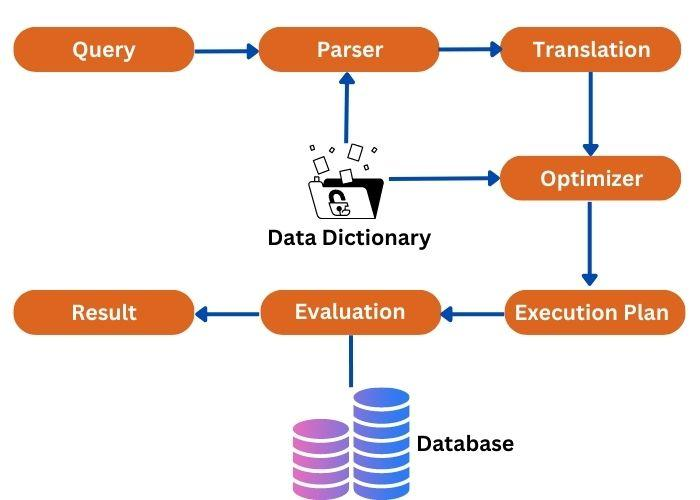
\includegraphics[width=0.5\textwidth]{Figure/Query processing.jpg}
    \caption{The flow of query processing in DBMS}
    \label{fig:my_image}
\end{figure}
    
    \item \textbf{Optimizer}: After parsing the query, the DBMS starts to find the most efficient way of executing the provided query. The factors for the query follow some optimization process. During the optimization stage, at least one complex parsing of one unique DML statement must be done. The database never optimizes DDL unless it includes a DML component, such as a sub-query, which needs optimization. Such operations are used for selecting data, inserting something, updating, etc. After everything is completed, then the evaluation step is made. in this step, the result is returned by the DBMS. This result is displayed to you in an appropriate format.
    \item \textbf{Result:} After getting the best execution plan, the DBMS starts the execution of the optimized query and perform the operation on data including selecting the data, inserting something, updating the data.\\
    Once everything is completed, DBMS returns the result after the evaluation step. This result is shown to you in a suitable format.\cite{Query,QueryProcessing,Oracle}
\end{enumerate}

\subsection{Query Optimization }When we write code, we aim for optimal logic in terms of both space and time complexity. Similarly, when we write database queries, we want them to be optimal in terms of their execution time and resource utilization's. Query optimization is  a crucial aspect of DBMS that seeks the most efficient way to execute a given query by considering a variety of query execution strategies. It minimizing the total cost or the total response time for the execution of a query.It is one of the factors that affect the application performance.\vspace{.4cm}

The result of a query is generated by processing the rows in a database in a way that yields the requested information. Since database structure are complex,in most cases and especially for not very simple queries, the needed data for a query can be collected from a database by accessing it  in different ways through different data structure and in different orders\cite{selinger-1979}. Each different way typically requires different processing time. Processing time of the same query may have large variance, from a fraction of a second to hours, depending on the chosen method. The purpose of a query optimization is to find the way to process a given query in minimum time, the large possible variance in time justifies performing query optimization, though finding the exact optimal query plan among all possibilities, is typically very complex, time consuming by itself may be too costly, and often practically impossible. Thus query optimization typically tries to approximate the optimum by comparing several common-sense alternatives to provide in a reasonable time.\vspace{.4cm}

There is a trade off between the amount of time spent figuring out the best query plan and the quality of the choice, the optimizer may not choose the best answer on its own. Different qualities of database management systems have different ways of balancing these two. Cost based query optimizes  evaluate the resource footprints of various query plans and use this as the basis for plan selection.These assign an estimated cost to each possible query plan and choose the plan with the smallest cost. Cost are used to estimate the runtime cost of evaluating the query, in terms of number of I/O operations required, cpu path length, amount of disk buffer space, disk storage service time, and interconnect usage between units of parallelism and other factors determined from the data directory. The set of query plans examined is formed by examining the possible access paths e.g. primary index, secondary index access, full file scan and various relational table join techniques e.g Merge join, Has join, Product join. the search space can become  quite large depending on the complexity of the SQL query. There are two types of optimization. These consist of logical optimization-which generates a sequence of relational algebra to solve the query-and physical optimization-which is used to determine the means of carrying out each operation.\cite{dremio-2024}


\subsubsection{Database query performance Metrics}
To effectively measure the performance of SQL queries, the following metrics are playing vital role. But most relevant metrics may vary depending on the specific database system and application requirements.
Here is a summery of key metrics used to evaluate and enhance query performance.\cite{chwesewicz-2024}
\begin{itemize}
    \item\textbf{Query execution time}: Total query duration to execute from start to finish. Measured in seconds or milliseconds. Lower execution time indicates better performance.
    \item\textbf{Query throughput}:It measures the number of queries or operation a database can handle per unit time, typically expressed as transaction per second (TPS) and queries per second(QPS)
    \item\textbf{Resource utilization}: Measures the percentage of time the cpu is occupied processing database operations. High cpu or memory usages can indicate heavy processing load or un-optimized queries.
\end{itemize}
\subsubsection{Key optimization techniques:}
 \begin{itemize}
     \item \textbf{Indexing}: Indexing is a crucial technique for query optimization in databases. It's named indexing because of how an index works in a book. An index is a structure that holds the field the index is sorting and a pointer from each record to their corresponding record in the original table where data is actually stored.\cite{tomar-2021,atlassian-no-date}
     \item \textbf{Query rewriting}: It is a technique that used in query optimization to transform a given database query into an equivalent form that executes more efficiently. It is one of the initial phases of query processing where original query is parsed and translated into an internal representation. This method particularly useful for complex queries, including those queries that have many sub queries or many joins.\cite{pitoura-2009,unknown-IBM-25-2024}
     \item \textbf{Partitioning}: This optimization method is specially  effective for large database. It involves splitting a large table or index into smaller segments to make the query more manageable pieces. Each partition acts as a separate entity that can be managed independently.\cite{planck-2024} 
     \item \textbf{Materialized view}: Materialized views are a powerful tool for query optimization, which we will focus on. 
 \end{itemize}
 
 \subsection{Reasons for Using Materialized Views for Query Optimization}:
\begin{itemize}
    \item\textbf{Precomputed result:} Materialized views store the results of a query that allows subsequent queries to access these precomputed results directly rather than recalculating them from the base tables. These results are updated periodically or on demand based on the underlying data changes.\cite{khan-2023,Risingwave-no-date}
    \item\textbf{Reduced Query complexity:} The main reason for creating materialized views is to improve query performance. It stores a snapshot of the data, that reduces the need for intricate query design, as we get the accesses precomputed results directly.\cite{Risingwave-no-date,Databricks-no-date}
    \item\textbf{Efficient use of resources:} As we  get the data from precomputed data and don't need to run full query every time materialized views decrease the computational load on database servers. It leads faster query response time and improved overall system performance and required fewer resources.\cite{google-no-date, khan-2023}
    
\end{itemize}\vspace{.4cm}

The motivation for using materialized views is to improve performance but the overhead associated with materialized view management can become a significant system management problem. The common materialized view management activities include: identifying which materialized view to create, indexing the materialized view; ensuring that all materialized views and materialized view indexes are refreshed properly each time the database is updated; checking which materialized views have been used; determining how effective each materialized view has been on workload performance; measuring the space being used by materialized views; determining which existing materialized views should be dropped,  archiving old detail and materialized view data that is no longer useful.\cite{Ashadevi2008CostEA,1363763}

\subsubsection{Challenges in query optimization} Query optimization is a crucial aspect of database management, aiming to improve the performance and efficiency of SQL queries.
\begin{itemize}
    \item\textbf{Data Fragmentation And Localization}: Dealing with how data is partitioned and distributed across multiple nodes. Data can be fragmented both horizontally and vertically and spread across nodes. Balancing between local execution and data transfer is also challenging. 
    \item\textbf{Query Decomposition and Allocation}: It refers to the process of breaking down a query into sub queries and assign them to different nodes.Challenging to choose best sub queries and node.
    \item\textbf{Complexity of Query Execution Plans}: Query optimization involves various techniques. Mastering these techniques can be challenging to find the most efficient one, especially for complex or multi-table queries.
    \item\textbf{Dependency On Indexes}: Proper indexing improves query performance but failing to create or maintain supporting indexes can result in inefficient query executions. Managing and updating indexes as data grows and changes can become a challenge.\\
    \cite{team-2020,etutorials-03-2024,editor-ijmter-2015}
\end{itemize}
\subsubsection*{Optimization Goals:}

\begin{itemize}
    \item Minimize response time
    \item Minimize resource consumption
    \item Minimize time to first tuple
    \item Maximize throughput
\end{itemize}\vspace{.4cm}
Expressed during optimization as a cost function. The common choice is to minimize response time within given resource limitations.



\subsection{What is a view in SQL:}
Views are perspective on a database. A view provides data of a database to a client and simultaneously prevents client access to the original database tables. When discussing views, the database tables always referred to as the view tables. View tables can reproduce the data of a database, they can provide a specific selection of data or they can compute new data out of the base table contents. Basically any analytical operation that can be derived from base table data can also be represented in a view table.\vspace{.4cm}

A view in SQL is a a virtual table that is generated by an SQL query. It does not store data physically but retrieves it from the underlying base table.Views are compiled at runtime, and they simplify the presentation of data from one or more tables without modifying the original data. It can be made over one or more database tables. Generally, we put those column in view that we need to query again and again. Once we created a view, we can make index, trigger on the view and query the view as table. A view may act as a filter on certain tables being referenced in the view \cite{chauhan-2024,Rohan_Vats-2024}

\subsubsection{Types of Views:}

There are two types of view in SQL server
\begin{itemize}
    \item \textbf{System defined view }: The system defined views are predefined views that already exists in the  master database of SQL server, such as tempdb, master and temp. Each of the database has its own properties and function. These system views will be automatically attached to any user-defined database.It will expose the metadata of the database and they can be used to get all possible information about the instance of SQL server or database objects, columns and contains. There are three types of System defined views, Information Schema, Catalog View, and Dynamic Management View. \cite{chauhan-2024}
    \item \textbf{User defined view }: This are the types of views that are defined by the user. User defined these view to meet their specific requirements.It can also divide into three types such as simple,complex and materialized views.\cite{javapoint-author-2024}
\end{itemize}
   
\subsection{Materialized Views }
 A special type of views are materialized views, It refers to that fact that the contents of the view are stored in form of a separate table, in the database system. MV are designed on the user requirements. A MV definition includes aggregation function like MIN, MAX, COUNT(DISTINCT),COUNT(*), SUM, AVG one or more table joined together and a GROUP BY operation doing on attributed and basic data definition language operation such as CREATE; ALTER and DROP may be applied on tables.\cite{Kardel_Thakare}. MV are a decision support/ data warehousing system tool that is able to increase by many orders of magnitude the speed of queries that access a large number of records.\cite{Kishan_Sainath} Nevertheless, materialized views can also be stored as a file or a data structure in-memory. Opposed to that a virtual view would be loaded from the base table in the moment it is requested. while the on-demand idea behind virtual views is certainly desirable.\cite{jan-no-date,ashadevi-2024}

\begin{definition}
Materialized views, also known as materialized tables or summary tables, are database objects that store the result of a query physically. Unlike regular views, which are virtual and compute their results on the fly, materialized views pre-compute and store the query results, allowing for faster retrieval and improved query performance.\\
Materialized views in databases optimize query performance by pre-computing and storing the result of complex queries involving aggregations and joins. This reduces the computational load during the execution, significantly speeding up the response times.

\end{definition}

A materialized view (sometimes called a sorted, projected and materialized view or SPM view) is a view whose columns have been sorted, projected and materialized.\cite{IBM} In database system optimize query performance by pr-computing and storing the result of complex queries involving aggregations and joins. As they store the results physically in a table re-computation to a query is not needed again. When it is view is already materialized at any time the same query is entered in the system. This reduces the computational load during the execution, significantly speeding up the response times.\vspace{.4cm}

Here's how they work:
\begin{itemize}
    \item\textbf{Pre-computations:} It store the results of queries that involve complex join and aggregations. These results are pre-computed and stored in database, reducing the time needed to fetch the data when required.
    \item\textbf{Storage and retrieval:} The data in materialized view is periodically refreshed to reflect changes in the underlying tables. The refresh can be scheduled or triggered by specific events, depending on the use case and requirements.
    \item\textbf{Refresh mechanism:}  Materialized views need to be refreshed to stay up to date with the underlying data.\vspace{.4cm}

    \begin{itemize}
        \item\textbf{Full Refresh:} The entire view is recomputed from scratch.
        \item\textbf{Incremental Refresh:} Only the changes since the last refresh are applied.
        \item\textbf{On Demand Refresh:} Triggered by specific events or user requests.
    \end{itemize}
\end{itemize}\vspace{.4cm}

Most of the time, the types of materialized views used are as follows:\vspace{.4cm}

\begin{enumerate}[label=\alph*)]
    \item \textbf{Materialized views with aggregates:} Materialized views with aggregates store the results of queries that perform aggregate calculations (e.g., SUM, COUNT, AVG, MIN, MAX) over large datasets. These views are particularly useful for optimizing query performance in scenarios that involve complex aggregations over vast amounts of data, such as reporting, analytics, and decision support systems. Example:
    
\definecolor{dkgreen}{rgb}{0,0.6,0}
\definecolor{gray}{rgb}{0.5,0.5,0.5}
\definecolor{mauve}{rgb}{0.58,0,0.82}
\lstset{language=SQL,
  basicstyle={\small\ttfamily},
  belowskip=3mm,
  breakatwhitespace=true,
  breaklines=true,
  classoffset=0,
  columns=flexible,
  commentstyle=\color{dkgreen},
  framexleftmargin=0.25em,
  frameshape={}{yy}{}{}, %To remove to vertical lines on left, set `frameshape={}{}{}{}`
  keywordstyle=\color{blue},
  numbers=none, %If you want line numbers, set `numbers=left`
  numberstyle=\tiny\color{gray},
  showstringspaces=false,
  stringstyle=\color{mauve},
  tabsize=3,
  xleftmargin =1em
}
         \begin{lstlisting}
 
CREATE MATERIALIZED VIEW SalesSummary
AS
SELECT
    ProductID,
    Region,
    CategoryID,
    SUM(SalesAmount) AS TotalSales,
    AVG(SalesAmount) AS AvgSales,
    COUNT(*) AS NumberOfSales
FROM Sales
GROUP BY ProductID, Region, CategoryID;

        \end{lstlisting}

    In this example, The materialized view "salesSummary" precomputes the Sum, AVG and COUNT for sales data grouped by ProductID, Region and CategoryID.

    \item \textbf{Materialized views with join }: Materialized views with joins store the results of queries that involve multiple tables combined using join operations (e.g., INNER JOIN, LEFT JOIN, RIGHT JOIN). These types of materialized views can significantly speed up complex queries that frequently access multiple related tables. By precomputing the join results, the materialized view avoids the need to recompute them during every query execution. Example: 
    
\definecolor{dkgreen}{rgb}{0,0.6,0}
\definecolor{gray}{rgb}{0.5,0.5,0.5}
\definecolor{mauve}{rgb}{0.58,0,0.82}
\lstset{language=SQL,
  basicstyle={\small\ttfamily},
  belowskip=3mm,
  breakatwhitespace=true,
  breaklines=true,
  classoffset=0,
  columns=flexible,
  commentstyle=\color{dkgreen},
  framexleftmargin=0.25em,
  frameshape={}{yy}{}{}, %To remove to vertical lines on left, set `frameshape={}{}{}{}`
  keywordstyle=\color{blue},
  numbers=none, %If you want line numbers, set `numbers=left`
  numberstyle=\tiny\color{gray},
  showstringspaces=false,
  stringstyle=\color{mauve},
  tabsize=3,
  xleftmargin =1em
}
         \begin{lstlisting}
CREATE MATERIALIZED VIEW CustomerOrderSummary
AS
SELECT
    c.CustomerID,
    c.CustomerName,
    o.OrderID,
    o.OrderDate,
    p.ProductID,
    p.ProductName,
    o.Quantity,
    o.TotalAmount
FROM
    Customers c
JOIN
    Orders o ON c.CustomerID = o.CustomerID
JOIN
    Products p ON o.ProductID = p.ProductID;

        \end{lstlisting}

    In this example, The materialized view "CustomerOrderSummary"
    stores the results of the joins between the customers, orders and products table.
    \item \textbf{Hybrid materialized views}: Hybrid materialized views combine features of both aggregate and join-based materialized views, optimizing performance for queries that require both aggregation and joins between multiple tables. They are designed to handle more complex queries efficiently, as they store precomputed results that involve both aggregated data and joined tables. Hybrid materialized views are particularly useful in environments like data warehouses or reporting systems where queries often need to summarize and relate data from various sources.
    \definecolor{codegreen}{rgb}{0,0.6,0}  % Green for comments
\definecolor{codegray}{rgb}{0.5,0.5,0.5}  % Gray for numbers
\definecolor{codepurple}{rgb}{0.58,0,0.82}  % Purple for strings
\definecolor{backcolour}{rgb}{0.95,0.95,0.92}  % Light gray background
\definecolor{bordercolor}{rgb}{0.7,0.7,0.7}  % Left border color (gray)
\definecolor{codeblue}{rgb}{0,0,0.8}  % Blue for SQL keywords

\lstdefinelanguage{MySQL}{
    keywords={SELECT, FROM, WHERE, JOIN, ON, INNER, OUTER, LEFT, RIGHT, FULL, GROUP, BY, ORDER, ASC, DESC, AS, COUNT, SUM, AVG, MAX, MIN, DISTINCT, INSERT, INTO, VALUES, UPDATE, SET, DELETE, CREATE, TABLE, PRIMARY, FOREIGN, KEY, DEFAULT, NULL, NOT, CHECK, CONSTRAINT, INDEX, VIEW, MATERIALIZED, PROCEDURE, FUNCTION, TRIGGER, DATABASE, ALTER, DROP, EXEC, IF, EXISTS, UNION, ALL, CASE, WHEN, THEN, ELSE, END, CAST, CONVERT, LIKE, IN, BETWEEN, AND, OR, HAVING, LIMIT, OFFSET},
    sensitive=false,
    morestring=[b]',  % String in single quotes
    morestring=[b]"   % String in double quotes
}

\lstdefinestyle{sqlstyle}{
    backgroundcolor=\color{backcolour},   
    commentstyle=\color{codegreen},  % Comments in green
    keywordstyle=\bfseries\color{codeblue},  % ✅ SQL Keywords in Blue & Bold
    numberstyle=\scriptsize\color{codegray},  % Row numbers in gray
    stringstyle=\color{codepurple},  % Strings in purple
    basicstyle=\ttfamily\footnotesize,
    breaklines=true,
    captionpos=b,
    numbers=left,      % ✅ Enables row numbers on the left
    stepnumber=1,      % ✅ Row numbers increment by 1
    firstnumber=1,     % ✅ Starts numbering at 1
    numbersep=8pt,     % ✅ Increases space between numbers and SQL code
    xleftmargin=3em,   % ✅ Ensures space inside the left border
    frame=single,      % ✅ Keeps a single border (left-aligned)
    framesep=5pt,      % ✅ Ensures space inside the frame
    rulesepcolor=\color{bordercolor},  % ✅ Matches row numbers with left border
    rulecolor=\color{bordercolor},  % ✅ Sets left border color
    language=MySQL  % ✅ Uses SQL keyword highlighting
}

\begin{lstlisting}[style=sqlstyle, caption={Hybrid materialized views}]

CREATE materialized VIEW productsalessummary
AS SELECT r.regionname,
          p.categoryid,
          p.productname,
          c.customerid,
          SUM(o.quantity)    AS TotalQuantity,
          SUM(o.totalamount) AS TotalSales
   FROM   customers c
          join orders o
            ON c.customerid = o.customerid
          join products p
            ON o.productid = p.productid
          join regions r
            ON c.regionid = r.regionid
   GROUP  BY r.regionname,
             p.categoryid,
             p.productname,
             c.customerid; 

\end{lstlisting}
This materialized view "ProductSalesSummary" stores precomputed join results between customers, orders, products and region as well as aggregate data total quantity and total sales.
    
\end{enumerate}

\subsubsection{Materialized view vs Database View:} With the usual syntax of creating a view, we create a database view  and that's different from the materialized view because a normal database view is just a virtual table that is defined by a SQL query. It is stored in the user database and can be accessed by user who have appropriate permissions. A MV view doesn't not store any data itself, it is simply  a way of presenting data from one  or more tables in different way. Materialized views are disk based and are updated periodically based upon the query definition.\cite{Stackoverflow-author-08-2008} Views are virtual and run the query definition each time they are accessed. Materialized views are useful when data is accessed frequently and updated infrequently.

 \subsubsection{ How materialized views work on MSSQL:} Not every database supports materialized views, and those that do each handle them a little differently, especially when it comes to the approach to view maintenance.\cite{hattemer-2020} Microsoft sql server supports materialized views, but they are called "indexed views" because a materialized view may be indexed in multiple ways and a materialization step is a matter of creating an index on a regular view. A view is materialized by creating a unique clustered index on an existing view. Uniqueness implies that the view output must contain a unique key. An indexable view must be defined by a single level SQL statement containing selections, inner joins and optional group-by.\cite{goldstein-2001}\vspace{0.8cm}

 To create a materialized views on mssql we have to create a  regular view and then a clustered index on the view:
 \begin{itemize}
     \item {Create a regular view with schemabinding:}

\definecolor{dkgreen}{rgb}{0,0.6,0}
\definecolor{gray}{rgb}{0.5,0.5,0.5}
\definecolor{mauve}{rgb}{0.58,0,0.82}
\lstset{language=SQL,
  basicstyle={\small\ttfamily},
  belowskip=3mm,
  breakatwhitespace=true,
  breaklines=true,
  classoffset=0,
  columns=flexible,
  commentstyle=\color{dkgreen},
  framexleftmargin=0.25em,
  frameshape={}{yy}{}{}, %To remove to vertical lines on left, set `frameshape={}{}{}{}`
  keywordstyle=\color{blue},
  numbers=none, %If you want line numbers, set `numbers=left`
  numberstyle=\tiny\color{gray},
  showstringspaces=false,
  stringstyle=\color{mauve},
  tabsize=3,
  xleftmargin =1em
}
         \begin{lstlisting}
CREATE VIEW schema_name.view_name
WITH SCHEMABINDING
AS
SELECT [columns]
FROM [tables]
WHERE [conditions]
GROUP BY [columns];

        \end{lstlisting}
The queries specify the schema and name of the view. With schemabinding options binds the view to the schema of the underlying tables. It prevents changes to the base tables that would affect the views definition.
      \item {Create a unique clustered index on the view:}
\definecolor{codegreen}{rgb}{0,0.6,0}  % Green for comments
\definecolor{codegray}{rgb}{0.5,0.5,0.5}  % Gray for numbers
\definecolor{codepurple}{rgb}{0.58,0,0.82}  % Purple for strings
\definecolor{backcolour}{rgb}{0.95,0.95,0.92}  % Light gray background
\definecolor{bordercolor}{rgb}{0.7,0.7,0.7}  % Left border color (gray)
\definecolor{codeblue}{rgb}{0,0,0.8}  % Blue for SQL keywords

\lstdefinelanguage{MySQL}{
    keywords={SELECT, FROM, WHERE, JOIN, ON, INNER, OUTER, LEFT, RIGHT, FULL, GROUP, BY, ORDER, ASC, DESC, AS, COUNT, SUM, AVG, MAX, MIN, DISTINCT, INSERT, INTO, VALUES, UPDATE, SET, DELETE, CREATE, TABLE, PRIMARY, FOREIGN, KEY, DEFAULT, NULL, NOT, CHECK, CONSTRAINT, INDEX, VIEW, MATERIALIZED, PROCEDURE, FUNCTION, TRIGGER, DATABASE, ALTER, DROP, EXEC, IF, EXISTS, UNION, ALL, CASE, WHEN, THEN, ELSE, END, CAST, CONVERT, LIKE, IN, BETWEEN, AND, OR, HAVING, LIMIT, OFFSET},
    sensitive=false,
    morestring=[b]',  % String in single quotes
    morestring=[b]"   % String in double quotes
}

\lstdefinestyle{sqlstyle}{
    backgroundcolor=\color{backcolour},   
    commentstyle=\color{codegreen},  % Comments in green
    keywordstyle=\bfseries\color{codeblue},  % ✅ SQL Keywords in Blue & Bold
    numberstyle=\scriptsize\color{codegray},  % Row numbers in gray
    stringstyle=\color{codepurple},  % Strings in purple
    basicstyle=\ttfamily\footnotesize,
    breaklines=true,
    captionpos=b,
    numbers=left,      % ✅ Enables row numbers on the left
    stepnumber=1,      % ✅ Row numbers increment by 1
    firstnumber=1,     % ✅ Starts numbering at 1
    numbersep=8pt,     % ✅ Increases space between numbers and SQL code
    xleftmargin=3em,   % ✅ Ensures space inside the left border
    frame=single,      % ✅ Keeps a single border (left-aligned)
    framesep=5pt,      % ✅ Ensures space inside the frame
    rulesepcolor=\color{bordercolor},  % ✅ Matches row numbers with left border
    rulecolor=\color{bordercolor},  % ✅ Sets left border color
    language=MySQL  % ✅ Uses SQL keyword highlighting
}

\begin{lstlisting}[style=sqlstyle, caption={Unique clustered index}]
CREATE UNIQUE CLUSTERED INDEX index_name
ON schema_name.view_name(column1, column2, ...);
\end{lstlisting}
This statement materialize the view and stores the result in a clustered index
\end{itemize}



 
\subsubsection{Deciding when to create a materialized view or a regular view}
There are some key factors to consider when deciding to create a materialized view or a regular view:\\
\textbf{Create a materialized view when all of the following are true}:
\begin{itemize}
    \item xxx
    \item xxx
    \item xxx
    \item xxx
\end{itemize}

\textbf{Create a regular view when all of the following are true}:
\begin{itemize}
    \item xxx
    \item xxx
    \item xxx
    \item xxx
\end{itemize}
 \subsection{Cost Model}
Materialized views are great optimization method. However, there is a cost associated with the jobs that maintain them.This section will discuss about the cost model of Materialized view.
 \begin{enumerate}[label=\alph*)]
    \item \textbf{Computing cost}: Computing cost mostly depends on the workload and data size. Query processing, data transferring, there are refresh mechanism to stay accurate. This all procedures are costly. Both the initial creation and subsequent refreshes of materialized views consume compute resources.
    \item \textbf{Maintenance cost}: This costs are associated with keeping Materialized views up-to-date and on service as base data changes. Every refresh or recalculation uses compute resources. Regular tuning, indexing, and monitoring to ensure the view optimally benefits query performance. The frequency of updates to base tables and complexity of the the materialized view impacts these cost. 
    \item \textbf{Storage cost}: Materialized views require additional disk space, particularly for large database.The storage cost of MV should be offset by the gain in query performance. Disabled views  still incur storage costs, even  they're not maintained or used for query optimization. As data volume grow, the storage costs for MV can increase significantly. This  aspect should be considered when designing a long term strategy for MV. 
    
    \item \textbf{Usage cost}
    
  Total cost= Query Execution savings-(Maintenance cost+ storage cost+ Freshens impact)

  Where:\\
  Query execution savings=Sum( Base query cost- MV cost)*query frequency \\
  Maintenance cost=refresh cost*refresh frequency\\
  Storage cost= MV size*storage unit cost\\
  freshness impact= Staleness penalty * query frequency.
 \cite{10.1145/2206869.2206874}\\
  
\end{enumerate}
 \subsection{ Static vs dynamic view selection }
\subsection{How  materialized views are different from normal tables in  SQL server }
\subsection{Conditions that must be fulfilled to be capable of using materialized views }

\subsection{ How Materialized view management and selection approach} :There are three types of materialized view that used to increase query performance and reduce the response time are as follows:

\begin{enumerate}[label=\alph*)]
    \item \textbf{Materialized view management task}
    \item \textbf{Materialized view selection}
    \item \textbf{Incremental Materialized View Maintenance}
\end{enumerate}

\subsection{Multiple View Processing Plans (MVPP) }
\subsection{Do all required rows exist in the views }
\subsection{Particle Swarm Optimization ( PSO ) Algorithm
 }
\subsection{Maintenance of existing materialized views (refresh)
}
\subsection{Materialized View Selection using (PSO) algorithm }
\subsection{Maintenance of existing materialized views (refresh)
}
\subsection{Do all required rows exist in the views }
\subsection{Fast filtering of MV}y